\documentclass[10pt]{article}        % twocolumn
%
\smartqed  % flush right qed marks, e.g. at end of proof
%
\usepackage{graphicx}
\usepackage[margin=15mm]{geometry}
\usepackage{subfig}
\usepackage[sort&compress]{natbib}
\bibpunct{[}{]}{,}{n}{}{}
\usepackage{epstopdf}
\usepackage{float}
%\usepackage{hyperref}
\usepackage{sidecap}
\usepackage{subfig}
\usepackage{epsfig}
\usepackage{amsmath}
\usepackage{caption}
\usepackage{color}
\usepackage{wrapfig}
\usepackage{tikz}

\usetikzlibrary{3d,calc,shapes,arrows}
\usetikzlibrary{patterns}
\usetikzlibrary{positioning}

\newcommand{\yslant}{0.5}
\newcommand{\xslant}{-0.6}

\pgfdeclareimage[height=0.8cm]{array}{Figures/microarray.png}



\begin{document}

\thispagestyle{empty}

	\scalebox{2.0}{
	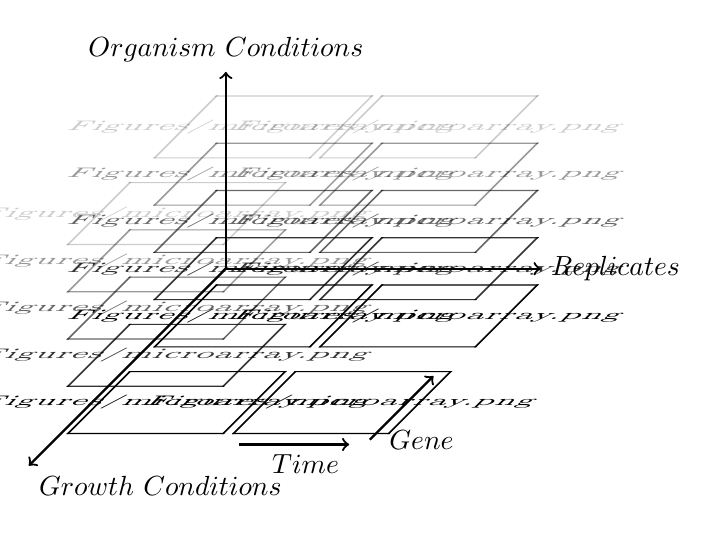
\begin{tikzpicture}
 	   \draw[thick,->,black] (0,0,0) -- (4,0,0) node[anchor=west ]{$Replicates$};
   	   \draw[thick,->] (0,0,0) -- (0,2.5,0) node[anchor=south]{$Organism~Conditions$};
  	   \draw[thick,->] (0,0,0) -- (0,0,6.5) node[anchor=north west]{$Growth~Conditions$};

   	 \node[] at (-0.6,-0.6) { \pgftext[at=\pgfpointorigin]{
            \pgflowlevel{\pgftransformcm{2}{0}{1}{1}{\pgfpoint{0}{0}}}
            \pgfuseimage{array}
            }};
     \node[opacity=0.80] at (-0.6,0) { \pgftext[at=\pgfpointorigin]{
            \pgflowlevel{\pgftransformcm{2}{0}{1}{1}{\pgfpoint{0}{0}}}
            \pgfuseimage{array}
            }};
     \node[opacity=0.60] at (-0.6,0.6) { \pgftext[at=\pgfpointorigin]{
            \pgflowlevel{\pgftransformcm{2}{0}{1}{1}{\pgfpoint{0}{0}}}
            \pgfuseimage{array}
            }};
     \node[opacity=0.40] at (-0.6,1.2) { \pgftext[at=\pgfpointorigin]{
            \pgflowlevel{\pgftransformcm{2}{0}{1}{1}{\pgfpoint{0}{0}}}
            \pgfuseimage{array}
            }};    
     \node[opacity=0.20] at (-0.6,1.8) { \pgftext[at=\pgfpointorigin]{
            \pgflowlevel{\pgftransformcm{2}{0}{1}{1}{\pgfpoint{0}{0}}}
            \pgfuseimage{array}
            }};         
            
   	 \node[] at (-1.7,-1.7) { \pgftext[at=\pgfpointorigin]{
            \pgflowlevel{\pgftransformcm{2}{0}{1}{1}{\pgfpoint{0}{0}}}
            \pgfuseimage{array}
            }};            
     \node[opacity=0.80] at (-1.7,-1.1) { \pgftext[at=\pgfpointorigin]{
            \pgflowlevel{\pgftransformcm{2}{0}{1}{1}{\pgfpoint{0}{0}}}
            \pgfuseimage{array}
            }};
     \node[opacity=0.60] at (-1.7,-0.5) { \pgftext[at=\pgfpointorigin]{
            \pgflowlevel{\pgftransformcm{2}{0}{1}{1}{\pgfpoint{0}{0}}}
            \pgfuseimage{array}
            }};
     \node[opacity=0.40] at (-1.7,0.1) { \pgftext[at=\pgfpointorigin]{
            \pgflowlevel{\pgftransformcm{2}{0}{1}{1}{\pgfpoint{0}{0}}}
            \pgfuseimage{array}
            }};    
     \node[opacity=0.20] at (-1.7,0.7) { \pgftext[at=\pgfpointorigin]{
            \pgflowlevel{\pgftransformcm{2}{0}{1}{1}{\pgfpoint{0}{0}}}
            \pgfuseimage{array}
            }};    

   	 \node[] at (1.5,-0.6) { \pgftext[at=\pgfpointorigin]{
            \pgflowlevel{\pgftransformcm{2}{0}{1}{1}{\pgfpoint{0}{0}}}
            \pgfuseimage{array}
            }};
     \node[opacity=0.80] at (1.5,0) { \pgftext[at=\pgfpointorigin]{
            \pgflowlevel{\pgftransformcm{2}{0}{1}{1}{\pgfpoint{0}{0}}}
            \pgfuseimage{array}
            }};
     \node[opacity=0.60] at (1.5,0.6) { \pgftext[at=\pgfpointorigin]{
            \pgflowlevel{\pgftransformcm{2}{0}{1}{1}{\pgfpoint{0}{0}}}
            \pgfuseimage{array}
            }};
     \node[opacity=0.40] at (1.5,1.2) { \pgftext[at=\pgfpointorigin]{
            \pgflowlevel{\pgftransformcm{2}{0}{1}{1}{\pgfpoint{0}{0}}}
            \pgfuseimage{array}
            }};    
     \node[opacity=0.20] at (1.5,1.8) { \pgftext[at=\pgfpointorigin]{
            \pgflowlevel{\pgftransformcm{2}{0}{1}{1}{\pgfpoint{0}{0}}}
            \pgfuseimage{array}
            }};   
     \node[] at (.4,-1.7) { \pgftext[at=\pgfpointorigin]{
            \pgflowlevel{\pgftransformcm{2}{0}{1}{1}{\pgfpoint{0}{0}}}
            \pgfuseimage{array}
            }};                               
      \draw[thick,->,black] (2.4,0,5.8) -- (3.8,0,5.8) node[anchor=north east]{$Time$};
  	   \draw[thick,<-] (4.1,0.1,3.8) -- (4.1,0.1,5.9) node[anchor=  west]{$~Gene$};       
    
	\end{tikzpicture}
	}
\end{document}